
% This LaTeX was auto-generated from MATLAB code.
% To make changes, update the MATLAB code and republish this document.

\documentclass{article}
\usepackage{graphicx}
\usepackage{color}

\sloppy
\definecolor{lightgray}{gray}{0.5}
\setlength{\parindent}{0pt}

\begin{document}

    
    \begin{verbatim}
c =[0.8 .8 .8];
im1 = 1*ones(25,25);
im2 = 1*ones(25,25);
im3 = 1*ones(25,25);
im4 = 1*ones(25,25);
im5 = 1*ones(25,25);
im6 = 1*ones(25,25);
for i = 1:World.NumStates
    [x,y] = find(World.StatesGrid == i);
    im1(x,y) = Net_NGMD.Node(3).Post(i,39)^.5;
    im2(x,y) = Net_NGMD.Node(3).Post(i,44)^.5;
    im3(x,y) = Net_NGMD.Node(3).Post(i,60)^.5;
    im4(x,y) = Net_NGMD.Node(5).Post(i,39)^.5;
    im5(x,y) = Net_NGMD.Node(5).Post(i,44)^.5;
    im6(x,y) = Net_NGMD.Node(5).Post(i,60)^.5;
end


figure;
subplot(5,3,1);
    imagesc(1-im1,[0 1]);
    colormap gray
    axis square
    hold on
    for k=1:6
        plot(Net_NGMD.Node(k).Pos(t,2),Net_NGMD.Node(k).Pos(t,1),'*','MarkerSize',10,'color','red');
    end
    hold off

subplot(5,3,2);
    imagesc(1-im2,[0 1]);
    colormap gray
    axis square
    hold on
    for k=1:6
        plot(Net_NGMD.Node(k).Pos(t,2),Net_NGMD.Node(k).Pos(t,1),'*','MarkerSize',10,'color','red');
    end
    hold off
subplot(5,3,3);
    imagesc(1-im3,[0 1]);
    colormap gray
    axis square
    hold on
    for k=1:6
        plot(Net_NGMD.Node(k).Pos(t,2),Net_NGMD.Node(k).Pos(t,1),'*','MarkerSize',10,'color','red');
    end
    hold off
subplot(5,3,4);
    imagesc(1-im4,[0 1]);
    colormap gray
    axis square
    hold on
    for k=1:6
        plot(Net_NGMD.Node(k).Pos(t,2),Net_NGMD.Node(k).Pos(t,1),'*','MarkerSize',10,'color','red');
    end
    hold off
subplot(5,3,5);
    imagesc(1-im5,[0 1]);
    colormap gray
    axis square
    hold on
    for k=1:6
        plot(Net_NGMD.Node(k).Pos(t,2),Net_NGMD.Node(k).Pos(t,1),'*','MarkerSize',10,'color','red');
    end
    hold off
subplot(5,3,6);
    imagesc(1-im6,[0 1]);
    colormap gray
    axis square
    hold on
    for k=1:6
        plot(Net_NGMD.Node(k).Pos(t,2),Net_NGMD.Node(k).Pos(t,1),'*','MarkerSize',10,'color','red');
    end
    hold off
subplot(5,3,[7 8 9]);
% [0 0 0 1 1 1 1 0 0 0 0 0 1 1 1 1 1 1 1 0 0 0 0 0 1 1 1 0 0 0 0 1 1 1 1 0 0 0 0 0 1 1 1 1 1 1 1 0 0 0 0 0 0 0 0 0 0 0 0 0 0 0 0 0 0 0 0 0 0 0 0 0 0 0]
hold on; area([3 6], [1 1],'FaceColor',c,'LineStyle','none');  area([12 18], [1 1],'FaceColor',c,'LineStyle','none');  area([24 26], [1 1],'FaceColor',c,'LineStyle','none');  area([31 34], [1 1],'FaceColor',c,'LineStyle','none'); area([40 46], [1 1],'FaceColor',c,'LineStyle','none');
p1 = plot(0:70,PM_NGMD_CEN.BCS(5,:)); p2 = plot(0:70,PM_NGCF_CEN.BCS(5,:));
xlabel('step')
ylabel('$D_B(P^*,\tilde{P}^3)$','Interpreter','Latex')
legend([p1 p2],'Hybrid','CF')

subplot(5,3,[10 11 12]);
hold on; area([3 6], [1 1],'FaceColor',c,'LineStyle','none');  area([12 18], [1 1],'FaceColor',c,'LineStyle','none');  area([24 26], [1 1],'FaceColor',c,'LineStyle','none');  area([31 34], [1 1],'FaceColor',c,'LineStyle','none'); area([40 46], [1 1],'FaceColor',c,'LineStyle','none');
p1 = plot(0:70,PM_NGMD_CEN.BCS(3,:)) ; p2 = plot(0:70,PM_NGCF_CEN.BCS(3,:));
xlabel('step')
ylabel('$D_B(P^*,\tilde{P}^5)$','Interpreter','Latex')
legend([p1 p2],'Hybrid','CF')

subplot(5,3,[13 14 15]);
hold on; area([3 6], [1 1],'FaceColor',c,'LineStyle','none');  area([12 18], [1 1],'FaceColor',c,'LineStyle','none');  area([24 26], [1 1],'FaceColor',c,'LineStyle','none');  area([31 34], [1 1],'FaceColor',c,'LineStyle','none'); area([40 46], [1 1],'FaceColor',c,'LineStyle','none');
p1 = plot(0:70,PM_NGMD_CEN.meanBCS);  p2 = plot(0:70,PM_NGCF_CEN.meanBCS);
xlabel('step')
ylabel('$\mathbf{E}(D_B(P^*,\tilde{P}^i))$','Interpreter','Latex')
legend([p1 p2],'Hybrid','CF')
\end{verbatim}

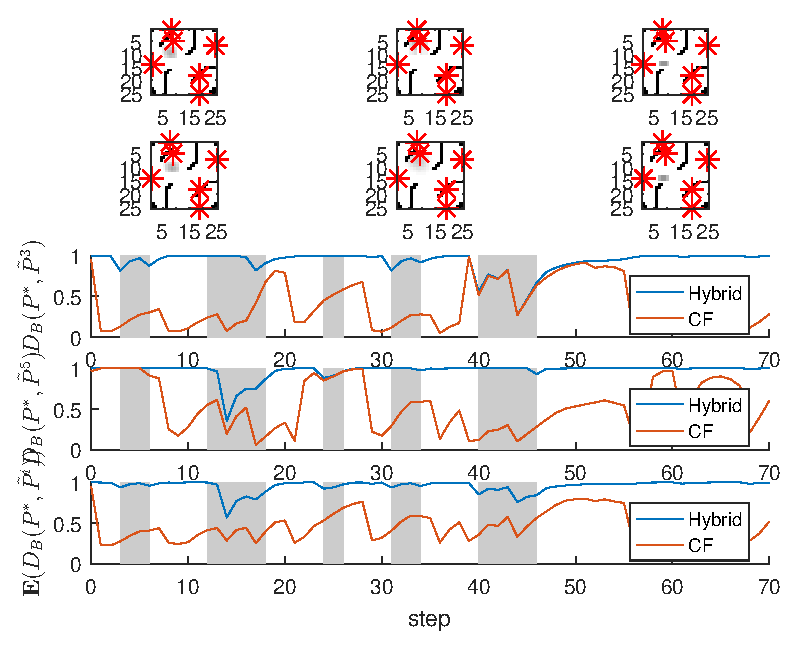
\includegraphics [width=5in]{Untitled_01.eps}



\end{document}
    
